\documentclass[titlepage]{article}
\usepackage[dvips]{graphicx}
\usepackage{html} 

\def\freeswan{{\bf FreeS/WAN}}
\def\pluto{{\bf Pluto}}
\def\code#1{{\tt #1}}


\author{Michael C. Richardson\\
	Sandelman Software Works Inc.\\
	On behalf of FreeS/WAN\\
	{\tt mcr@sandelman.ottawa.on.ca}}
\date{\today}
\title{FreeSWAN KLIPS version 2 requirements and implementation schedule}

\begin{document}
\maketitle\newpage

\section{Executive Summary}

\begin{verbatim}
$Id: klips2req.tex,v 1.1 2001/11/27 03:49:30 mcr Exp $
\end{verbatim}

This is a plan for evolution of current FreeSWAN KLIPS code into ``next
generation'' KLIPS code. A review of requirements and applicability to
intended design is presented, followed by a review of current KLIPS1
architecture.

The target architecture is then described.

A plan both to develope this document and to transition from old to new is
presented.

%This document contains a list of desired requirements, including decision as
%to relative importance of these. A schedule for development of a plan to
%consense on these requirements is presented. 

\section{Current KLIPS input/output structure}

\subsection{output: ipsec\_tunnel\_start\_xmit}

\begin{enumerate}
	\item gather private information
	\item clone skb if necessary
	\item verify that packet is IPv4
	\item compute hard header length
	\item decrement TTL
	\item lookup in erouting table
	\item UDP port 500 exception
	\item start encapsulation loop
	\begin{enumerate}
		\item check for DROP or missing eroute
		\item check for REJECT eroute
		\item check for PASS eroute
		\item check for HOLD eroute
		\item check for TRAP eroute, signal PF\_KEY, swap to HOLD eroute
		\item acquire lock for walking tdb chain
		\item calculate headroom required for chain
		\begin{enumerate}
			\item check if SA is in larval, drop
			\item check if SA is dead, drop
			\item check if replay overflowed, expire SA
			\item check if lifetime counters have overflowed, expire SA
			\item switch on protocol type, to calculate headroom size.
			\begin{enumerate}
				\item if ESP switch on protocol type to calculate tailroom size.
			\end{enumerate}
		\end{enumerate}

		\item calculate mtudiff, send ICMP fragment needed. Mark ``note2''

		\item hack MSS if desired

		\item copy upper (layer 2) header to safety if it was present

		\item check if data fits in existing skb, else expand.
		\item apply grouped transforms
		\begin{enumerate}
			\item apply disaster of \#ifdefs.
			\item switch by protocol type, calculate headroom for this stage
			\begin{enumerate}
				\item if ESP, then switch by cipher get headroom
				\item if ESP, then switch by hash to get tailroom
			\end{enumerate}
			\item double check (not in NDEBUG) if there is enough headroom
			\item push the data ahead
			\item double check (not in NDEBUG) if there is enough tailroom
			\item extend the data behind
			\item see if packet has become too long (bigger than 64K)
			\item finally move the plaintext as appropriate
			\item switch on protocol type
			\item case: ESP
			\begin{enumerate}
				\item switch on cipher type, prepare IV
				\item prepare self-describing padding
				\item switch on cipher type, do encryption
				\item switch on cipher type, update IV
				\item switch on hash type, do authentication
			\end{enumerate}
			\item case: AH
			\begin{enumerate}
				\item prep replay info, headroom
				\item switch on hash type, do authentication
			\end{enumerate}
			\item case: IPIP, apply encap
			\item case: IPCOMP
			\begin{enumerate}
				\item call skb\_compress
				\item do some debugging
			\end{enumerate}
			\item recalculate header checksum
		\end{enumerate}
		\item lookup eroute by new outer header, if we found
			something and the src/dst have changed
	\end{enumerate}
	\item send ICMP if packet has become too big
	\item re-apply link layer header if there was one.
	\item attempt to re-route the packet
	\item drop packet if new route leads to us again.
	\item do connection tracking
	\item do netfilter localout output call
	\item call ip\_send or IP\_SEND depending on kernel version
\end{enumerate}

\subsubsection{Comments upon problems/limitations of transmit}

\subsection{input: ipsec\_rcv}

\begin{enumerate}
	\item increment module use count
	\item verify skb and data is not NULL
	\item verify hard header length
	\item clone (COW) if necessary
	\item a number of poorly documented ``assertions''
	\item verify protocol number against packet and against protocol structure
	\item verify that protocol is AH, COMP or ESP.
	\item lookup each ipsecX device to determine which one has been bound 
		to the receiving device. Grab ipsecprv device info.
	\item if no device found, warn, but do not die
	\item begin decap loop
		\begin{enumerate}
		\item lock tdb if this is first time through
		\item verify that length is appropriate multiple if ESP
		\item switch on protocol type, grab SPI value from appropriate place
		\item format sa with satoa. (not found in code)
		\item if AH, then determine AH header length, find next protocol value, and
			verify against expected length of AH header.
		\item get spin lock if required
		\item if IPCOMP
		\begin{enumerate}
			\item check if IPCOMP is out most header, (not yet supported)
			\item advance the tdb pointer and, if doing inbound policy
				check, then check SPI value. Complain if not matched.
			\item decompress packet, reset ip header pointer to new
				value, loop (via continue) 
		\end{enumerate}
		\item lookup tdb based upon SA. \code{gettdb}
		\item complain if no tdb
		\item if doing inbound policy check
		\begin{enumerate}
			\item check that outer source matches one on packet.
			\item check that this tdb is the expected next from
				previous. (forward check) 	
			\item check that this tdb expects to be attached to
				previous. (reverse check) 
		\end{enumerate}
		\item check if tdb state is larval, skip
		\item check if tdb state is dead, complain
		\item check lifetime (bytes - soft/hard, addtime - soft/hard, usetime -
			soft/hard, packet count - soft/hard). Expire TDB,
			tell pfkey if limit exceeded.
		\item pick authlen, switch on auth type (MD5, SHA1)
		\item switch on protocol type (ESP, AH only) and set up authenticator
		\item check sequence number to see if replay window rolled, if so expire
		\item check out replay window, dropping if it is a replay
		\item verify authenticator, check if there was
			authentication, switch on type 
		\begin{enumerate}
			\item MD5, call MD5Update and friends, checking if
				ESP or AH was involved 
			\item SHA1, call SHA1Update and friends, checking if ESP or
				AH was involved	 
			\item none, do nothing
		\end{enumerate}
		\item check authenticator for NULL (which would imply not AH
			or ESP above) 
		\item compare authenticator against hash, complain if failed
		\item update the replay window
		\item switch on protocol type
		\begin{enumerate}
			\item if ESP
			\begin{enumerate}
				\item switch on encryption algorithm
				\begin{itemize}
					\item if 3DES, then find IV and set header length
					\item otherwise, fail
				\end{itemize}
				\item locate ciphertext based upon header length
				\item switch on encryption algorithm
				\begin{itemize}
					\item if 3DES, verify data length
						multiple of 8 and decrypt. 
					\item no otherwise clause
				\end{itemize}	
				\item find next header type
				\item find padding 
				\item verify padding
			\end{enumerate}
			\item if AH, do nothing
		\end{enumerate}
		\item update protocol number in header (why?)
		\item switch on protocol type
		\begin{enumerate}
			\item if ESP, the memmove as appropriate for ESP,
				skb\_pull() to compact, and then skb\_trim.
			\item if AH, then memmove as appropriate for AH, skb\_pull().
		\end{enumerate}
		\item update skb pointers to parts of packet.
		\item nuke any options that skb knew about, or skb->proto\_priv (2.2+)
	\end{enumerate}
	\begin{enumerate}
		\item recalculate the header checksum
		\item set the sbk protocol type to IP over ethernet
		\item advance tdb pointers
		\item if doing inbound policy check
		\begin{enumerate}
			\item verify that backward policy agrees with forward policy
			\item check if next protocol field is not one we know about
			\begin{enumerate}
				\item complain that policy was not complete
			\end{enumerate}
		\end{enumerate}
		\item update ipcomp ratio counters if IPCOMP was involved, but this
			stage is not IPCOMP
		\item update the lifetime values in bytes, packets, and last used
			time.
		\item loop again if ESP, AH or IPCOMP
	\end{enumerate}

	\item if original chain was IPCOMP, then advance tdb chain once (Why?)
	\item if there is one last tdb
	\begin{enumerate}
		\item verify that last protocol type was IPIP (no transport
			supported here)
		\item if doing inbound policy checks
		\begin{enumerate}
			\item advance tdbnext with inext, and complain if
				non-NULL. (i.e. check that this was last tdb)
			\item verify source IP address matches tdb source
		\end{enumerate}
		\item update lifetimes for this tdb
		\item if skb data len is too small for header length,
			complain
		\item pull up new header into skb
		\item advance ip pointer to inner header
		\item update raw header pointer
		\item zero protocol options
		\item update layer 2 protocol info to IP over Ethernet
		\item reset checksum info
	\end{enumerate}
	\item if we are doing EROUTE checking (i.e. tunnel exit checking)
	\begin{enumerate}
		\item setup for look up by src/dst in eroute table, checking
			for IPIP header.
%		didn't we already advance ipp above? why are we looking in
%		a tunnel that we didn't make?
		\item lock eroute table, lookup eroute
		\item record info we need and unlock
		\item if we found what we need, then lock, and lookup policy
			information by new said block.
		\item if no tdb found, then we drop packet
		\item walk policy\_tdb chain, look for last one
		\item compare against tdb that we just used, complain if not
			the same.	
	\end{enumerate}
	\item unlock tbd
	\item update stats if appropriate
	\item release packet destination 
	\item if there was a layer 2, copy it back into place
	\item do inbound policy checks if it was IPCOMP 
% WHY HERE?
	\item do connection tracking
	\item drop packet back into bottom half queue
\end{enumerate}

\subsubsection{Comments upon problems/limitations of receive}

\section{KLIPS1 static structure}

\begin{figure}
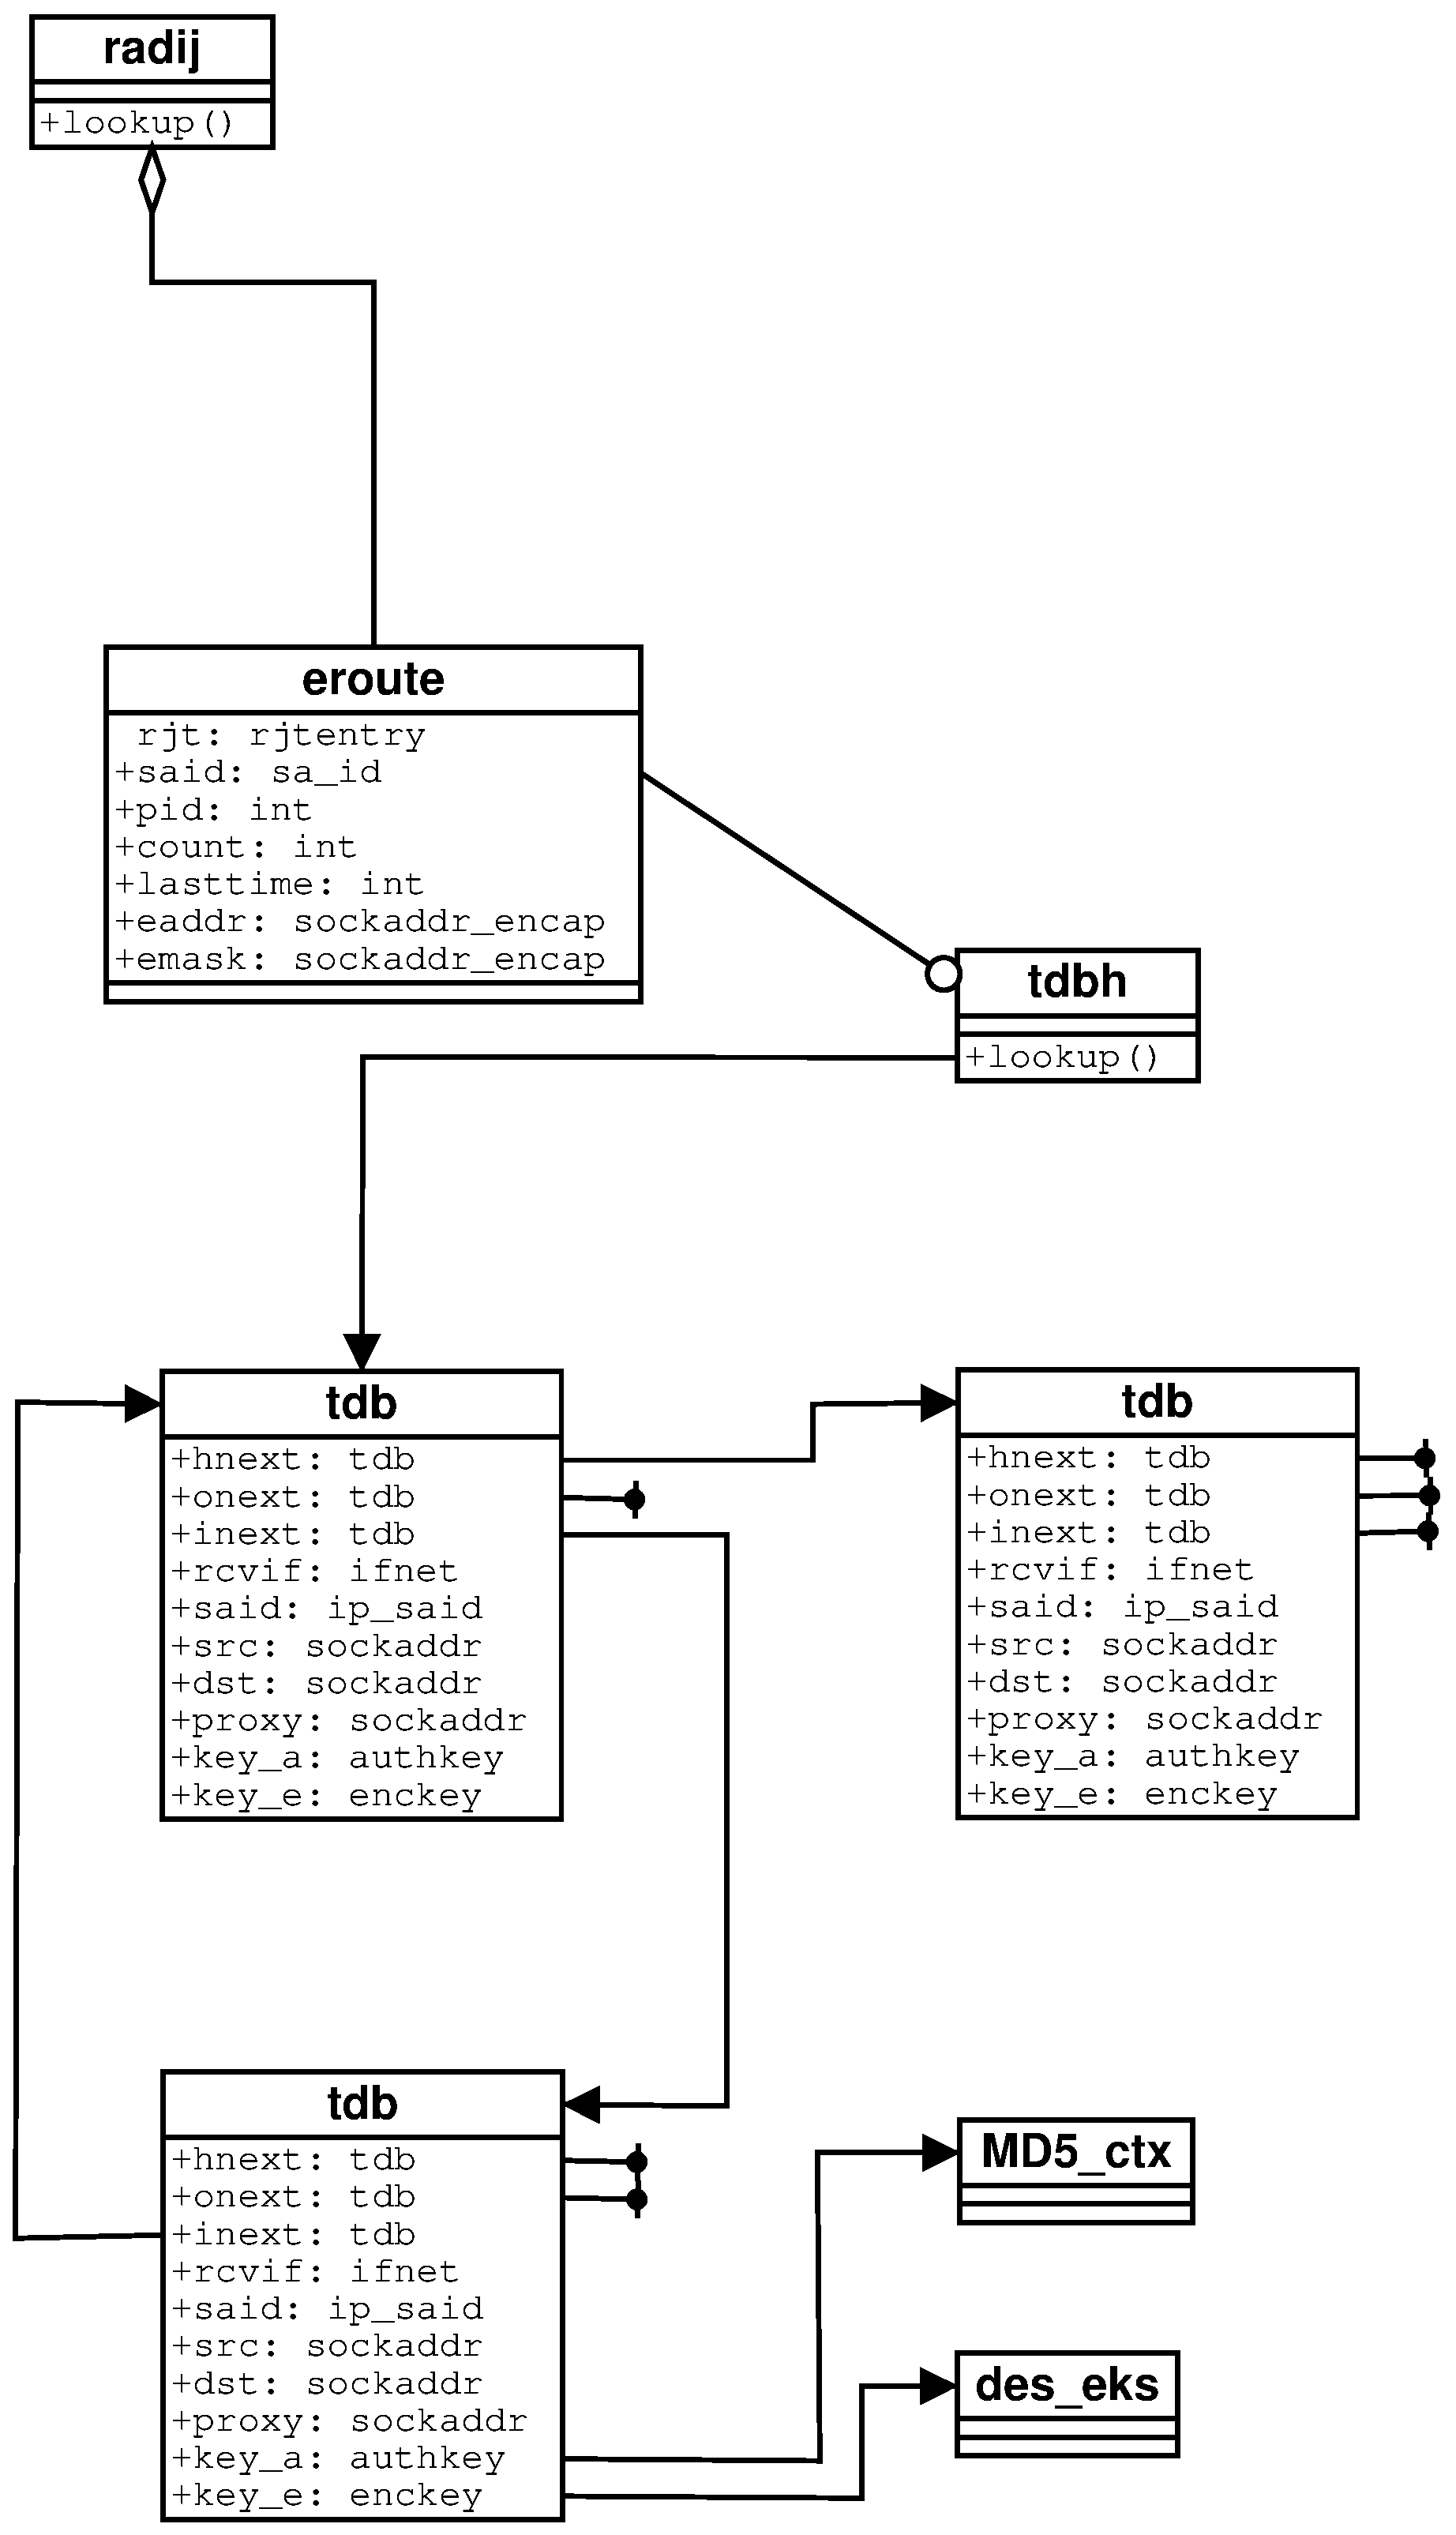
\includegraphics[height=6in,width=6in]{diagrams/klips1_tdb.eps} 
\label{KLIPS1 structures}
\end{figure}

\subsection{klips1 radij}

The \code{radij} module is an adaptation of the BSD \code{radix.c} code. It
has been consistently renamed to as to coexist with \code{radix.c}. It
implements a netmask aware patricia tree on blocks of data.

An explanation explains that the pronounciation is almost the same since the
``j'' is to be pronounced like the Greek chi.

\subsection{klips1 eroute}

An eroute entry describes an entry in the security policy database. The
\code{eroute} currently only includes selectors for source and destination address.

\subsection{klips1 tdbh}

This is an array of pointers to \code{struct tdb} structures. It serves as
a root for chained hash buckets. It is an open hash.

These are managed by the code in \code{ipsec\_xform.c}. These provide a
mapping from a \code{struct sa\_id} to a \code{struct tdb} based upon SPI,
protocol and destination address. 

The entries in each bucket are linked together using the \code{tdb\_hnext}
field.

\subsection{klips1 tdb}

This structure represents all the information associated with a single
transform. In the case that multiple transforms may be chained together, they 
are chained together using \code{tdb\_inext} and \code{tdb\_onext}. The ``i''
and ``o'' are short for inner and outer. Thinking of the resulting packet as
an onion, these pointers describe transforms towards the {\bf i}nner and {\bf 
o}uter directions.

\subsection{klips1 md5\_ctx}

This stores the key context for the MD5 authentication routines. This
structure is different from the \code{MD5\_CTX}, in that this is the HMAC
version and contains an inner and outer \code{MD5\_CTX}.

\subsection{klips1 sha1\_ctx}

This block is not shown in the diagram, but serves an analogous function to
\code{md5\_ctx}. 

\subsection{klips1 des\_eks}

This block contains a DES key schedule (this is not equivalent to a DES key,
but has been scheduled already). Note that this is really a container
and is assumed to be of the proper size. The DES routines actually take a
\code{des\_cblock} as input.



	
	
		
		
	
	


\section{Detailed Requirements}
\label{detailreq}

\subsection{001: changeable gw wild-side addresses on-the-fly}

\subsubsection{001: Definition of requirement}

Some systems use DHCP or IPCP (PPP) to get an address assigned. DHCP in
particular has a clear lease time, and at the end of the lease, a different
IP address may be assigned. 

The requirement is for \freeswan\ to interact with address assignment
facilities, adjust lifetime parameters appropriately, and to transparently 
change systems with the address change.

\subsubsection{001: response}

The movement away from a layered device model means that KLIPS should not
interfere with this process. Most of the issues should be on the key
management side (\pluto\ ).

The specific requirements for pluto are that it is willing to listen to
the routing socket so that it can learn about new interfaces, and about
routes. If there is no route to the remote IKE daemon, then there is no point 
in attempting to initiate.

Further, consider the case where our wild-side address {\em changes}.  
We need a hook so that pluto is notified so that it can notify all the
affected peers. 

The peers need to change the outer-header destination address on all packets
destined for us.  And in the general case, this requires rekeying the affected tunnels.  
(Future specification may in fact make this unnecessary, but pre-existing
peers will continue to exist)

The specific requirements for the startup script are that the default
route (or any routes for that matter) need not exist to permit the ``conn'' to
be configured.

See also requirement 4.

This requirement is useful for Opportunistic Encryption.




\subsection{002: address inertia}

\subsubsection{002: Definition of requirement}

The essence of this requirement is that gateway's can remember where the
wild-side address of road warriors are. Should a reboot (or a restart of
\pluto\ ) occur, it would re-initiate to these clients.

There are three levels of support which may be desireable:

\begin{enumerate}
\item[Level 1] 	record only the wild-side address for re-initiation.

\item[Level 2]  record the wild-side address, and all current phase 1 (DH and
			SKEYID) keying materials.

\item[Level 3] 	record the wild-side address, and phase 1 and phase 2 keying materials.
\end{enumerate}

\subsubsection{002: response}

Satisfaction of level 1 of this requirement will require changes only to 
\pluto, specifically to provide a way to get a list of current connections,
to record this in a stable file, and a for the boot up scripts to read the
alternate list of configurations as well. So, this requirement can be
satisfied without impact to KLIPS2 design.

Level 2 of this requirement has some issues. The storage of keying material
on disk may be a source of concern. This issue would need to be addressed
in the design. The source of this requirement is to provide reliable recovery
and fast reboots, systems that involve operator intervention may not satisfy
this. The chief advantage of storing the phase 1 information is that it
reduces the amount of time required to do DH exponentiation after a reboot. 
A new phase 2 would have to be done as well.

Level 3 of this requirement has further issues. It requires some help from
KLIPS2 to provide for the retrieval of keying materials (including replay
state) from the kernel, and subsequent reloading of it. There are clearly
even more issues with making sure that the materials are not inappropriately
revealed. 
In addition, the state of eroutes, filtering, etc. will need to be
captured. Saving of this information may have very strong advantages in the
opportunistic case, as the information on whether or not to set up an
opportunistic tunnels is valuable as well. Further, in the opportunistic
case the risk of disclosure of the keying material may be considered low
enough that storing it is worthwhile.

In all three cases, there is a cost-benefit analysis to do, weighing the
improvements in reliability and performance against the risks of
inappropriate disclosure. The answer to this analysis may always be a local
matter. 

In addition, all three cases would apply to restarting of \pluto\ either on
purpose (to facilitate easy updates), or due to program error (core dump).

There are further legal issues. Access to the keying materials may facilitate 
cooperation with law enforcement access. This is not regarded as a feature.

Opportunistic encryption would benefit from any amount of key maintenance.
Road warriors are the ones most likely to benefit as they are turned
off/suspended most often. However, their wildside address is also most likely 
to change, rendering any saved state that they have useless.

\subsection{003: mini-database of road warriors that persists across reboots}
\subsubsection{003: Definition of requirement }

This requirement appears to be a repeat of requirement 001.




\subsection{004: connection up, down, wanted}

\subsubsection{004: Definition of requirement }

All internal SA entries should have a status of whether the connection is up
(keying material is available), down (keying material has expired), or is
wanted (keying material not yet available). This is part one.

There is an additional situation in which the MAST device may need to be
marked down. This is when it is known by the routing system that all routes
to the outer destination will fail. This will typically only be true for
systems without default routes (i.e. that are in a default-free zone). This
second feature is part two.

\subsubsection{004: Response}

Part one is committed to. There is an issue that we currently do not 
look for expired SAs unless we are attempting to use them. To fix this,
we will need to walk the SA table periodically. 

Part two raises some design questions. Specifically, how does one know if
the outer destination is routable unless looks?

\begin{itemize}
\item each SA (and thus each conn) could maintain a pointer to
   a struct dst\_entry. This has some savings in that one doesn't
   have to lookup the route each time that the SA is used.
   (One does the lookup if the entry is either invalid, or non-existant,
   this is just a cache. The TCP PCB does this as well)

   As these structures are reference counted, we can safely hang
   on to this.

   If asked about link status of a MAST device, then one just has to walk
   all SAs associated with this device, looking for at least one with SA
   which has not been obsoleted.

\item alternatively, we do as we currently do, but upon failure to find
   a route to the outer dst, we bash the link status of the device to
   down. (We only change when all SAs say down, which makes this somewhat
   difficult)

   Once the device is down, then we should really discard any packets that
   arrive at the MAST device. We do not want to waste time encrypting things
   we would then through away. 

   We could do something like let 1\% through to do the above test, but that
   seems like a poor choice, since routing daemons may have found other ways
   around in the meantime, so no traffic would ever reach us.

\end{itemize}

See also requirement 1.

The first solution is preferred, but neither are committed to at this time.



     







\subsection{005: routing below tunnel layer to support mobility and multi-homing}

\label{req005}

\subsubsection{005: Definition of requirement }

Ciphertext packets should be treated like all other packets, and should be
subject to normal routing proceedures.

\subsubsection{005: Response}

Implementation of MAST devices and packet escalator should accomplish this.

This is a critical piece for reliability of opportunistic encryption, as
current routing tricks cause plaintext packets to blackhole after a physical
interface flap.



\subsection{006: SAs entries should be capable of overlapping}

\subsubsection{006: Definition of requirement }

Currently klips1 apparently identifies a tunnel by what {\bf remote} subnet it 
serves.  That means that if a new tunnel is brought up serving the same 
subnet, it supersedes the previous one.

A more complex semantic is required, and a way to express it:

\begin{itemize}
\item sometimes you do want the new tunnel to supersede the old one.
\item sometimes you want the new tunnel to operate in parallel, using 
	equal-cost multipath, for load sharing.
\item sometimes you want the new tunnel to just sit there in standby mode, 
	to be used later
\begin{itemize}
\item for fail-over
\item for mobililty
\end{itemize}
\end{itemize}

\subsubsection{006: response}

This is a misfeature, and is hereby deprecated.

Rollover of SAs is necessary for functional long-term opportunism.

%Possibly constructive suggestion (to be filed under some OTHER 
%heading):  We could have family lineages:  Within each family lineage, 
%parents would be replaced by children as the former expire.  They would 
%keep the "family name".  The name could be derived perhaps from the name of 
%the CONN declartion in the .conf file.
%
%To implement load-sharing, mobility, and failover, we could have multiple 
%families serving the same remote subnet.





\subsection{007: why do equalizing schedulers not play well with tunnels?}

\subsubsection{007: Definition of requirement }

linux/net/sched/sch\_teql.c says:

\begin{verbatim}
    1. Slave devices MUST be active devices, i.e., they must raise the tbusy
       signal and generate EOI events. If you want to equalize virtual devices
       like tunnels, use a normal eql device.
\end{verbatim}

A normal ``eql'' device ({\tt linux/drivers/net/eql.c}) simply does a simple
form of round-robin scheduling among devices. It can round robin among
devices of equal weight.

The teql scheduling device uses the scheduling system's back pressure (the
{\tt dev->tbusy} flag) to give each device as much as it wishes.

\subsubsection{007: response}

The KLIPS1 {\tt ipsecX} devices are never busy. They therefore can not be
equalized using this scheduler.

The virtual devices could use the {\tt tbusy} mechanism. To be able to
do this, the {\tt MAST} device will have to be given a clear amount of
resources on a per-virtual device basis. As the limit to throughput will be
the lesser of encryption throughput and physical device throughput, once the
buffers are full, the virtual device can raise the {\tt tbusy} flag.

For this to be useful, the paths to the remote host must be
different. Specifically, the outer destination address must in some way be
different. If there are simply two physical ways to get to the same
destination address then standard load-balancing would work once the 
{\tt MAST} devices have processed the cleartext.

The use of the {\tt tbusy} feature is not considered to contribute strongly
towards Opportunistic Encryption. The creation of the MAST device is however
critical.
 



\subsection{008: decouple SA retrieval from DADDR (don't care how it arrived)}

\subsubsection{008: Definition of requirement }

The desire is that the SA lookup by SPI should not depend upon destination
address. This is in contradiction to IPsec requirements, but an
implementation that assigns unique SPI numbers to all protocols can satisfy
both requirements.

This requirement also helps NAT traversal in some cases.

\subsubsection{008: response}

As SPI values are assigned by the receiver for unicast, we can in general
accomplish this by allocating all SPI values from a single pool. This is
committed to.

This is neutral towards Opportunistic Encryption.



\subsection{009: SPIs unique, independant of protocol and DADDR}

\subsubsection{009: Definition of requirement }

This is a variation of requirement \#8. 
\subsection{010: routing above tunnel layer}

%  3.1   Multiple Tunnels to Same Subnet
%   
%   Suppose  West is a FreeS/WAN box that is connected to two different wild-side ISPs. It has
%   two  different  wild-side  addresses.  It  would be very nice to set up two connections to
%   Sunrise-net.  This  would  allow load-sharing, and it would also improve reliability if we
%   could arrange failover from one connection to the other.
%   Unfortunately,  if  you  try  to  set  up multiple connections to the same subnet (Sunrise
%   subnet)  using  FreeS/WAN  version  1,  the result is fratricide. The second connection is
%   treated as a replacement for the first.
%   You  can  work  around this by not making subnet connections. Instead, as suggested by Joe
%   Patteson,   make   host-to-host   connections   between   East  and  West,  and  then  run
%   GRE-encapsulated  traffic  over  these  connections,  as discussed in section 2.2. You can
%   perform load-balancing and failover with respect to the GRE virtual devices.
%   If East has N ISPs and West has M ISPs, you could conceivably want M�N IPsec connections.
%   Note the following imperfect parallelism:
%     * IPsec  tunnel  mode  is  sometimes  described (imperfectly) as follows: Set up an IPIP
%       tunnel, and then apply transport-mode encryption to the encapsulated traffic.
%     * In  this  case,  we encapsulate using GRE, and then apply transport-mode encryption to
%       the encapsulated traffic.
% 
%    On  the  other  hand,  it is not 100% correct to view tunnel mode as IPIP plus encryption,
%  because  real  tunnel  mode  allows allows the system to verify that the correct subnet is
%   being  carried  over  the  tunnel; that is, the inner headers can be checked. In contrast,
%   using  IPIP+encryption  or GRE+encryption, the inner headers are just data in some obscure
%   format that cannot be checked by the IPsec system per se.
%   On  the  third  hand,  since  FreeS/WAN relies on you, the user, to implement the security
%   policy  anyway,  using the firewalling system, you can perfectly well check the packets as
%   they enter the GRE device. So all the necessary functionality can be achieved.
%   Also  note that the GRE links, as the name implies, were designed with routers in mind, so
%   their up/down state is meaningful, and their metric is meaningful to routing daemons.
%   It  sure  would  be nice if the next-generation IPsec system could do this itself, without
%   requiring  us  to  resort  to  GRE.  We  need  multiple  tunnels  to the same subnet, with
%   meaningful  up/down  state  and  meaningful  metrics. And we need the ipsec device to play
%   nicely with routing daemons.
   
  

\subsubsection{010: Definition of requirement }

%   http://www.quintillion.com/fdis/moat/ipsec+routing/
%especially section 3 therein, i.e.
%   http://www.quintillion.com/fdis/moat/ipsec+routing/#sec-routing-above
%
%That was written over a year ago.  The big ideas haven't changed, but a few 
%details need polishing.
%  *) In particular, there are several places where it speaks of a "device" 
%going down whereas is should say "link" going down.
%
%  *) Also the rationale is given in terms of failover and load-sharing, and 
%we now know that mobility is a third important motivator for doing this.
%
%  *) Also the terminology
%         a) routing above the tunnel
%         b) routing below the tunnel
%has been deemed unnecessarily confusing to Muggles.  It would be better to 
%speak of
%         a) routing the inner headers (plain text)
%         b routing the outer headers (crypto text)
%but the intended meanings are unchanged.
%
%===========
%
%Tangentially relevant remark: Routing above the tunnel is one of the big 
%motivations for having a virtual device.  A detailed look at how this might 
%work, as worked out at OLS, was posted to the list at 02:15 PM 7/30/01 -0400.

see JSD documents.


\subsection{011: granularity smaller than host}

\label{req011}

\subsubsection{011: Definition of requirement }

It is desired to do SPD lookups based upon UDP/TCP port numbers (source and
destination) as well as source and destination address.

In addition, for hosts a lookup based upon Unix UID should be possible.

For gateways, it is also desirable to do lookup based upon IPSO labels.

\subsubsection{011: response}

UDP/TCP port number lookups will be present in the second release of KLIPS2.

IPSO labels will be present in the third release of KLIPS2.

This feature will not contribute to Opportunistic Encryption.




\subsection{012: /dev/ipsecNNN devices that could be chown(1)ed and chmod(1)ed.}

\subsubsection{012: Definition of requirement }

One of the grand ideas of Unix is the notion that ``everything is a file''.  

As a result, network devices don't show up in /dev/ in a useful way, and they
don't have file-modes and file-owners.  Instead you need to deal with them
using special commands like {\bf ifconfig}, and special system calls like
{\bf bind, setsockopt, ...}

As a result, it is clear how to establish an IPsec connection from host A to 
host B, but it is really not obvious how to establish an IPsec connection 
from user UX (process PX) to user UY (process PY).  

Could a user have his own ipsec.conf file?  
How would that file be related to the system's ipsec.conf file?

Even if the user doesn't have his own ipsec.conf file, how do we implement 
per-user or per-process tunnels?  I can imagine what the kernel code looks 
like to enforce the restrictions, but what does it look like to the user 
process?  Making it look like a named pipe with a file-owner and some 
file-permissions is one way... that makes it look more like good-old "core" 
unix but less like other networking stuff.  

\subsubsection{012: response}

Constructive proposals would be most welcome.

This feature is not committed to in any form at this time.





\subsection{013: process to process tunnels}

\subsubsection{013: Definition of requirement }

The idea here goes something like this:  User IDs are a clumsy form of 
identification and authentication.  Modern systems do much better.  

For instance, using ssh, one can have one window (one process group) for
which one has started an ssh-agent which holds one's certificates.  

One can have another window logged in under the same user ID, but with
different certificates, or indeed no certificates at all.  

This is the modern approach:  security resides in the keys, not in the user IDs.

User IDs have a clear meaning locally.
They have only a weak relationship on relationship to entities on a distant
system.

Certificates do have meaning as anyone with a public key in a trusted store
with clear authorizations attached can trust some entity that has the 
corresponding private key.

\subsubsection{013: response}

During the definition stage of "granularity finer than per-host", (such as
in requirement \#11) it will be necessary to clearly articulate what the
appropriate size of a "grain" will be.

No specific programming work is committed to for satisfaction of this
requirement, rather a step in the process for definition of requirement \#11
has been made. 












\subsection{014: ways to manipulate tunnel perms.}

netfilter, pf\_key, ioctl, $/dev/ipsecNNN$ 

\subsubsection{014: Definition of requirement }

This is a variation of the question \#13: how do user applications request
security services from the kernel. 






\subsection{015: KLIPS as a loadable module (isn't it already?)}

\subsubsection{015: Definition of requirement }

The KLIPS system should permit compilation as a loadable module to permit easy
intregration.

\subsubsection{015: response}

This requirement is currently met in KLIPS1, and will be retained for future
work.

While LKM is a permitted configuration, it must always be possible to compile 
the module statically.



\subsection{016: stats: (number,time\_of\_last) packets (out,good\_in,error\_in)}

\subsubsection{016: Definition of requirement }

Each SA bundle should maintain a list of statistics. 
This should include:

\begin{enumerate}
\item number of packets encapsulated
\item time last used to encapsulate
\item number of packets decapsulated properly
\item time last used to decapsulate properly
\item number of packets decapsulated improperly
\item time last used to decapsulate improperly
\end{enumerate}

\subsubsection{016: response}

These numbers will be maintained. Appropriate locking granularity needs to be
determined.

This feature must be designed in properly for it to work, and is therefore
of priority.


\subsection{017: integrate IPsec and firewall policy into Security Policy.}

\subsubsection{017: Definition of requirement }

To provide industrial-strength security, the IPsec Security Policy Database
should be integrated with the regular Linux firewalling facilities,
specifically into the Netfilter/IPtables code. 

Integration provides a single place to express policy.
It prevents duplication of code: this is both a savings in physical
quantities (kernel time and code space) as well as a reduction in
opportunities for errors.

\subsubsection{017: response}

This is a core design requirement for KLIPS3.

As I said at OLS (see Claudia's notes, posted to this list at 11:04 AM 
8/1/01 -0400)...  Any form of IPsec *requires* proper firewall rule 
management.  IPsec security is (and always has been, and always will be) 
totally dependent on this.

People think that bringing up a tunnel creates security.  This is 
diametrically wrong.  Real life is always a tradeoff between security and 
functionality.  A tunnel creates new functionality;  it creates a new path 
for packets to flow.  Security comes when AND ONLY WHEN you close down the 
old insecure paths.

The IPsec rfcs require IPsec to have a Security Policy Database.  "The form 
of the database and its interface are outside the scope of this 
specification."  according to section 4.4.1 in
   http://www.ietf.org/rfc/rfc2401.txt

But some nontrivial semantics is required.  Just bringing up a tunnel (a 
"virtual wire") is !not! sufficient to comply with the letter or the spirit 
of this rfc.  IPsec !must! provide the IPsec-administrator with some means 
to express a security policy that cuts off the bad old insecure paths.

The tricky part comes when we try to integrate the tunnel-related policies 
with whatever other policies the admin might have in mind.

=======

To look at it from a slightly different viewpoint:  Everybody who installs 
freeswan will be able to express an ultra-vague ultra-high-level security 
objectives:  they want all the good things to happen, and they want none of 
the bad things to happen, whatever that means.

At the ultra-low level, the kernel provides some tools for allowing and 
disallowing various packet flows based on various criteria.

The problem is that there is a huge disconnect between the high-level 
objectives and the low-level tools.  The low-level stuff has a lot of 
changeable details:
  -- the details change on boot up:  rc.d/init.d/network start
  -- the details change on card insertion:  pcmcia/network start $dev
  -- the details change when DHCP runs....
  -- the details change when tunnels go up and down...
  -- the details might depend on what our routing daemons are telling us.

  *) Making this work is a royal pain in the neck or worse.
  *) Making it work robustion for redhat AND debian AND suse, etc. is an 
even bigger pain.
... but in my humble opinion this is a REQUIRED part of any real-world 
IPsec implementation.

The freeswan project has taken quite a firm stand on some other 
security-related issues such as single-DES.  I hope it will take an equally 
firm stand on implementing an industrial-strength Security Policy 
Database.  Single-DES is a joke, suitable for hobbyists only.  Tunneling 
without firewalling (etc.) is in the same category.




\subsection{018: full inbound policy checking}

\subsubsection{018: Definition of requirement }

Upon decryption/decapsulation of a packet, the inner set of selectors should
be checked against SA definition. This is a requirement from RFC2401. It
provides a paranoid check against possible mis-behaviour/mis-configuration of
a corresponding peer.

\subsubsection{018: response}

This will be present in the 1.92 release.

This facility will be present in the KLIPS2 design as an optional feature.


\subsection{019: secure ciphers and hashes}

\subsubsection{019: Definition of requirement }

The project will use only ciphers and hashes which are known to be secure.
The definition of secure used includes: that the algorithm has sustained a reasonable
length of analysis, that it can not be brute forced with current technology
in less than a decade, and that there are no covert channels.

\subsubsection{019: response}

Use of MD5, SHA1 as hashes and 3DES for cipher is currently used.
This will be maintained.

1DES is considered insecure and will not be added.
RC4 is considered insecure and will not be added.

The project will only add new algorithms after extensive discussion.
AES is currently under discussion, but is not scheduled to be added at this
time.





\subsection{020: kernel implementation (should be faster)}

\subsubsection{020: Definition of requirement }

Appropriate benchmarks are sought to live up to.


\subsection{021: plays well with routing daemons}

\label{req021}

\subsubsection{021: Definition of requirement }

In order to provide for appropriate interaction with routing daemons, a
logical interface is required to which to anchor routes. The keying status of 
the connection should be reflected in to the link status of the logical
interface.

\subsubsection{021: response}

The proposed MAST device satisfied this requirement, and is a defining
feature of KLIPS3.


\subsection{022: free of export restrictions}

\subsubsection{022: Definition of requirement }

Many countries have placed restrictions on what their citizens may do, or
having done this, may restrict who the product may be given to. The project's 
code should not be encumbered in this manner.

\subsubsection{022: response}

The project will continue to refuse contributions from residents or citizens
of the United States of America. The recent changes to the administration of
the BXA are not sufficient cause change this policy as they may change again
very quickly.



\subsection{023: standard crypto api to add newer ciphers and hashes}

\subsubsection{023: Definition of requirement }

The current KLIPS1 encapsulation and decapsulation routines make explicit
synchronous calls to the 3DES encrypt and decrypt functions. This causes
three problems:
\begin{enumerate}
\item it makes it difficult to add new algorithms, both at compile time and
	at runtime.
\item it fails to make use of multiprocessor systems effectively
\item it fails to interface nicely to hardware acceleration devices
\end{enumerate}

A standard API from FreeSWAN KLIPS to algorithm functions (e.g. 3DES-MD5-ESP)
would provide for plug and play capabilities for algorithms.

An asynchronous interface would permit multiple processors or hardware
accelerators to interface easily as well.

Despite this, the packets must still emerge from the system in the same order 
that they arrived. That is, they must not be reordered, as this causes
inefficiencies for TCP.

\subsubsection{023: response}

A design to use an asynchronous interface to algorithms will be provided as
part of KLIPS2.

The design proposed by Bart Trojanowski (rsa1) <bart@jukie.net> will be used
as a basis.


\subsection{024: opportunistic}

\subsubsection{024: Definition of requirement }

\subsubsection{024: response}

This is a core goal of FreeSWAN.



\subsection{025: SADB hash table will be locked for additions/deletions}

\subsubsection{025: Definition of requirement }

The SADB table will have a fine grained lock.





\subsection{026: use a refcount on each SA to increase locking granularity}

\subsubsection{026: Definition of requirement }

Each SA object will use reference counts to determine when it may be freed.

The SAs will be referenced from eroute's via an indirection table, reducing
the need to search by SAID, yet not introducing new pointers that may not be
easy to find. This same index will occur in {\tt skb->nfmark} references.








\section{Proposed data architecture}

\begin{figure}
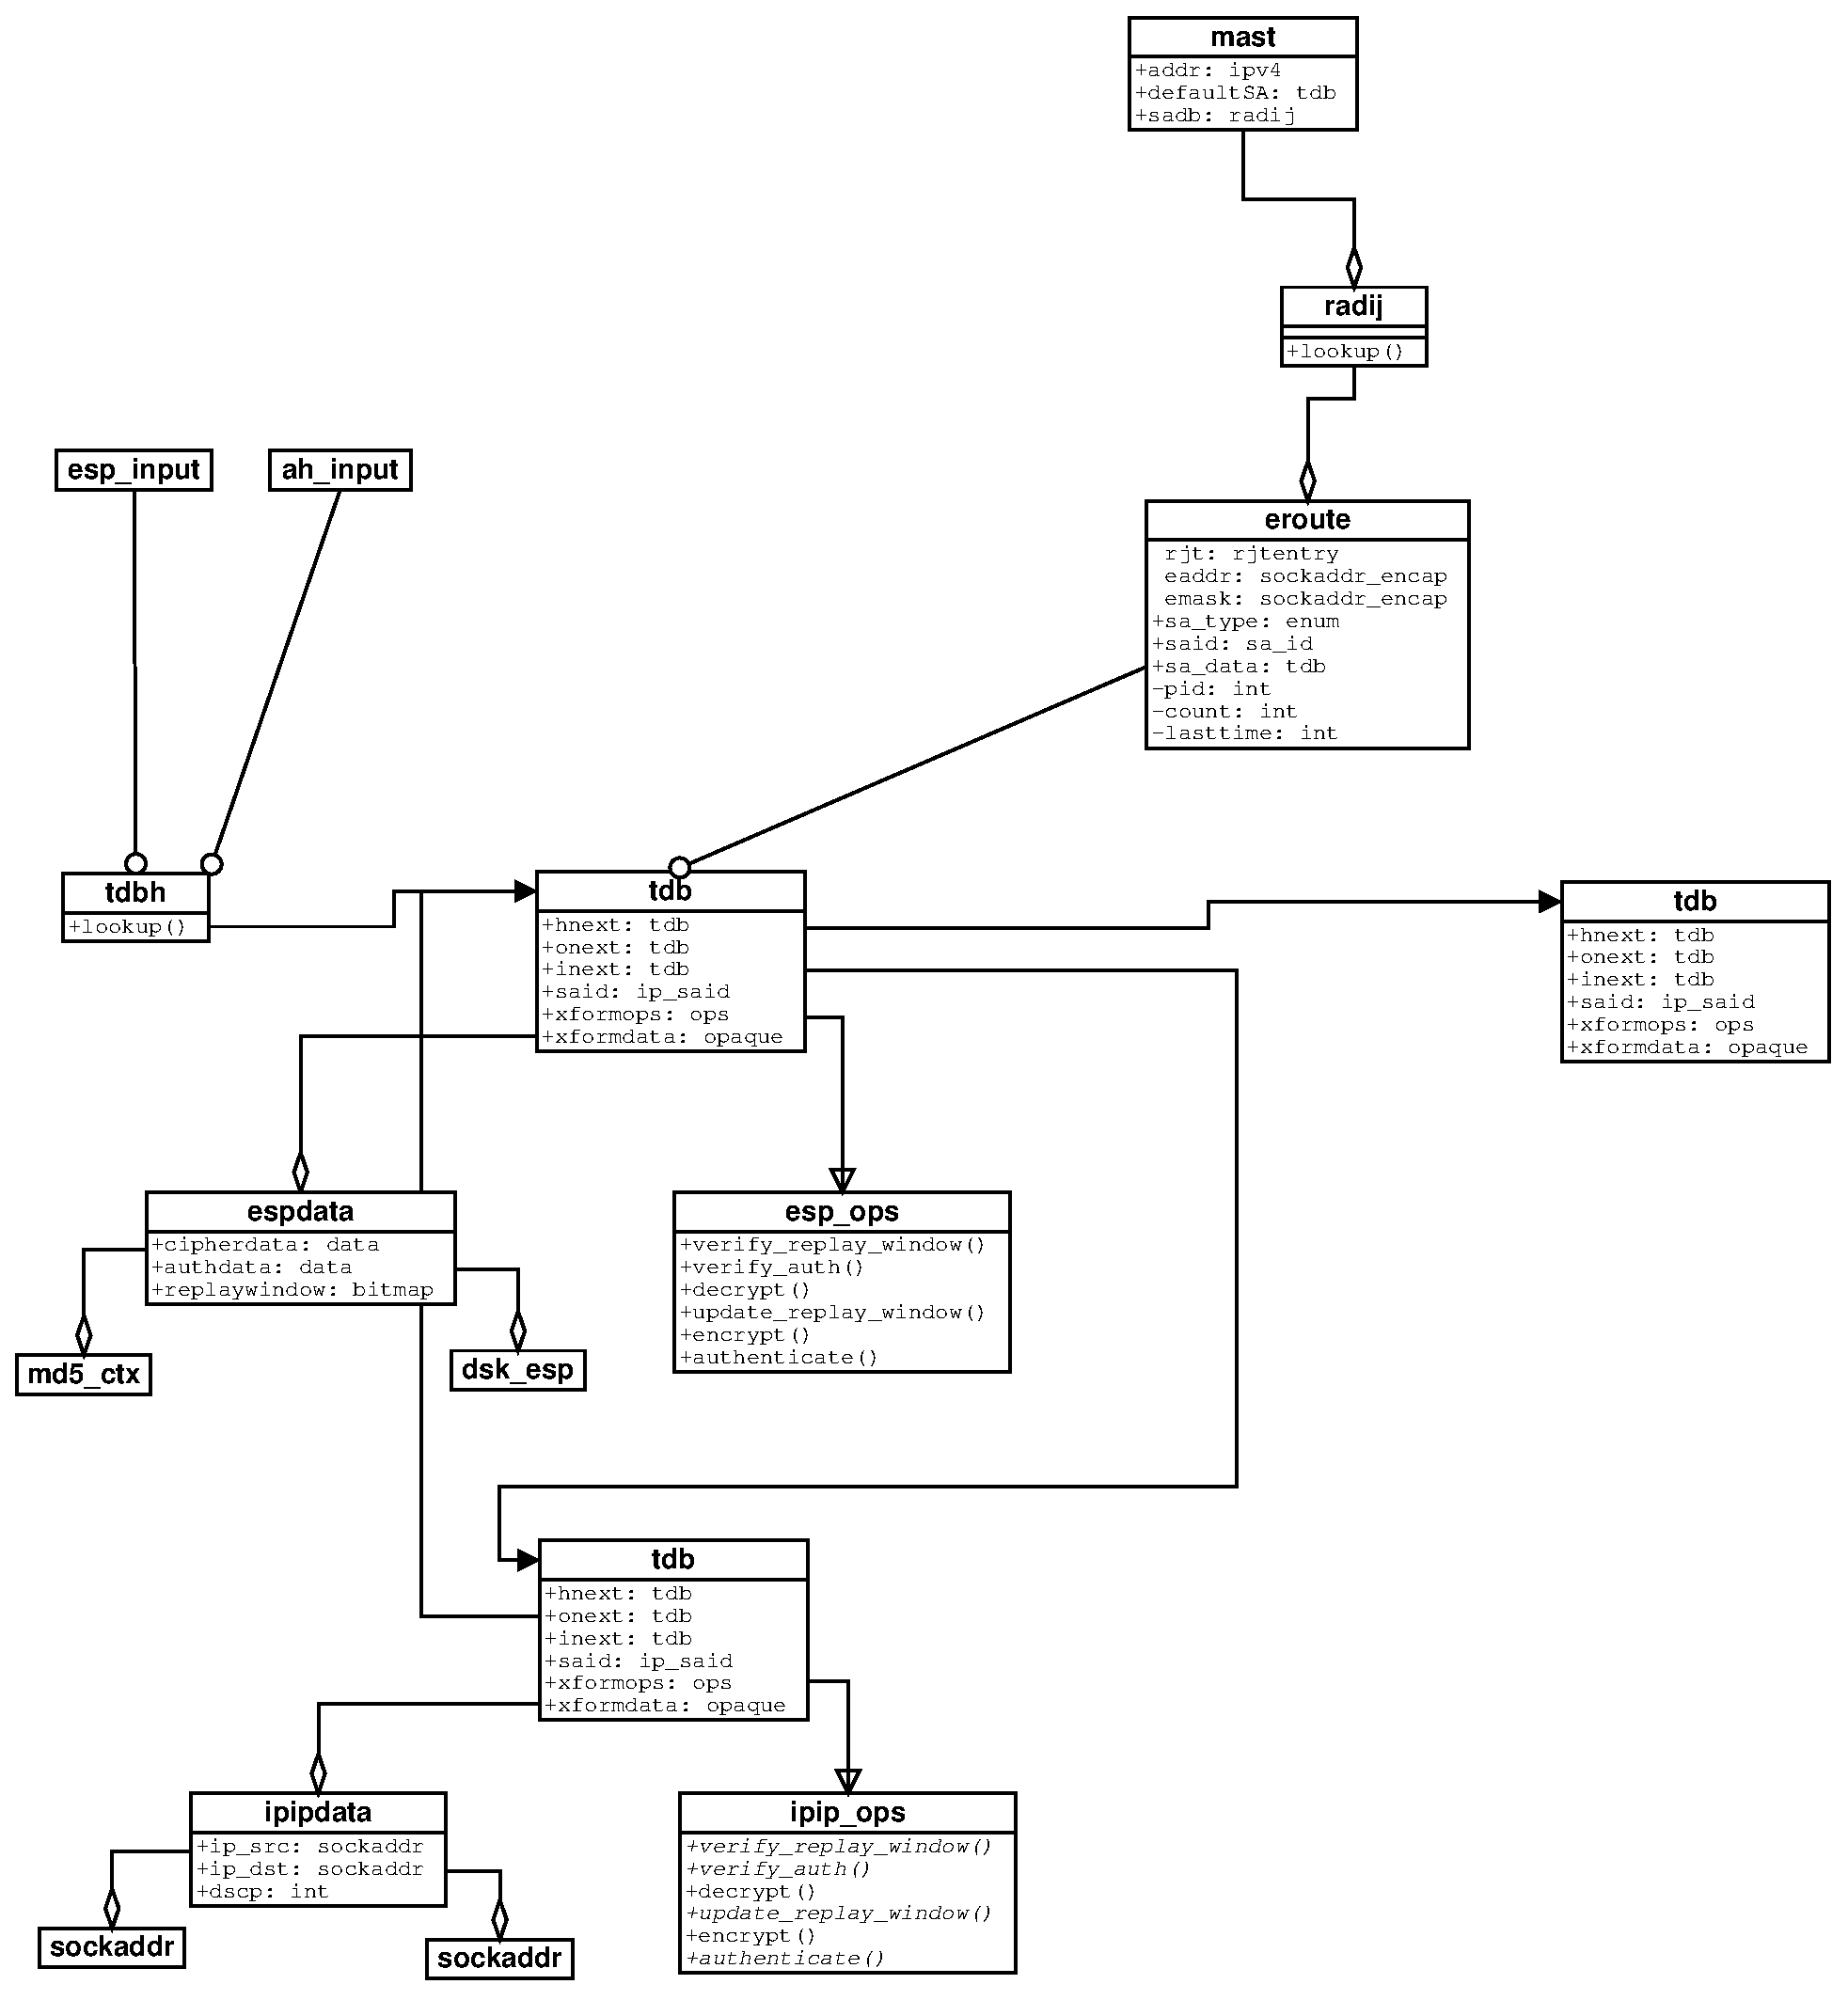
\includegraphics[height=6in,width=6in]{diagrams/klips2_tdb.eps} 
\label{KLIPS2 data structures}
\end{figure}

\subsection{klips2 mast}

The MAST device provide a mooring point for routing protocols and firewall
policies. The MAST device represents one or more IPsec tunnels. 

Packets routed to a MAST device will get encrypted with a default SA.
A different SA may be specified using NetFilter (aka ipchains, aka iptables)
rules. 

Packets that are received via one of the SAs associated with this device
will be marked as having been received on a MAST device. 

The link status of a MAST device reflects the keying status of all underlying 
SAs. If at least one SA is keyed, then the MAST device will be up. If no SA
that is associated has valid keys, or if no SAs that are associated with the
device, then the device will be marked down.

This is provided in part to satisfy requirement 21 (see \ref{req021})
and requirement 5 (see \ref{req005}).

\subsection{klips2 radij}

The radij tree provides a lookup on eroute entities.  

While the eroute database provides the IPsec security policy database (SPD),
the radij tree is the index into it by selectors.

It is a BSD radix.c derived table. It has been modified to permit masking of
bits of the index to occur in arbitrary places, thus permitting both source
and destination addresses to be masked.

The radij tree will be replaced or augmented to support additional selectors.
These include UDP/TCP port numbers, SPI numbers (for multiple layers of
gateways), ICMP types and codes, and possibly also IPSO labels.

As opportunistic encryption creates large numbers of fully specified
source/destination pairs, it will be investigated if an auxiliary table could
provide a more efficient storage of these tables. Specifically, it is
possible that connection tracking can more efficiently provide this required
index. 

\subsection{klips2 eroute}

The eroute is the object that represents an entry in the IPsec SPD.

This structure will be extended with additional selectors to support
requirement 11 (see \ref{req011}).

\subsection{klips2 ipsec\_sa\_buckethead}

This is the root of the transform database hash table. 

This structure is the renamed {\tt tdbh}.

\subsection{klips2 esp\_input}

The current {\tt ipsec\_rcv} will be cloned to create an ESP receive
function.

\subsection{klips2 ah\_input}

The current {\tt ipsec\_rcv} will be cloned to create an AH receive function.

\subsection{klips2 ipsec\_sa}

This is the renamed {\tt tdb} structure.

\subsection{klips2 espdata}

This is a per-SA structure that records all the information needed by the
algorithm database functions to perform their functions.

\subsection{klips2 esp\_ops}

This is the set of pointers to functions needed to perform the ESP steps.

\subsection{klips2 md5\_ctx}

This is a subpiece of the espdata structure that stores MD5 keys.

\subsection{klips2 ipipdata}

This structure provides information needed by the IPIP transform.

\subsection{klips2 ipip\_ops}

This is the set of pointers to functions needed to perform IPIP steps.


\include{milestones}

\end{document}

